% %%%%%%%%%%%%%%%%%%%%%%%%%%%%%%%%%%%%%%%%%%%%%%%%%%%%%%%%%%%%%%%%%%%%%%
% Dummy Chapter:
% %%%%%%%%%%%%%%%%%%%%%%%%%%%%%%%%%%%%%%%%%%%%%%%%%%%%%%%%%%%%%%%%%%%%%%

% %%%%%%%%%%%%%%%%%%%%%%%%%%%%%%%%%%%%%%%%%%%%%%%%%%%%%%%%%%%%%%%%%%%%%%
% The Introduction:
% %%%%%%%%%%%%%%%%%%%%%%%%%%%%%%%%%%%%%%%%%%%%%%%%%%%%%%%%%%%%%%%%%%%%%%
\fancychapter{Implementation}
\label{cap:implement}


The implementation presented in this paper was created by utilizing the generic indoor location system presented in section \ref{sec:architecture} and applying it with bluetooth low energy. The system's architecture is presented in figure ~\ref{fig:implementation} and is divided three parts: the bluetooth low energy device, in section ~\ref{subsec:beacon} a description of the used technologies and the changes made are present;the server, whose funcionalities and stored information are described in section ~\ref{subsec:server}; and the smartphone application, whose process is described in section ~\ref{subsec:app} alongside figures that show the functional prototype. For each of these parts an explanation will be given, containing a description of each of its components specific to the presented system alongside the requirements for each to work.


This chapter gives an overview of the state of the art of Indoor positining solutions. The \acf{BLE}'s architecture and functionality is analyzed in section \ref{sec:ble}, while section \ref{sec:indoortech} overviews the other existing technologies. The most common techniques utilized for position computation along side examples which make use of them are explained in section \ref{sec:techniques}. Finnally on section \ref{sec:related} analyzes the most projects that had the most relevance in the field and the existing work related to \ac{BLE}.

\section{ \ac{BLE} beacons}
\label{sec:beacon}


The beacons that were utilised are Texas Instruments CC2650STK devices which can be visualised in figure ~\ref{fig:beacon}. Alongside the device, which comes with a pre-installed bluetooth low energy program capable of giving information on each of its ten sensors through its predefined profiles, there is a texas smartphone application that can connect to a single device and read from its sensors. By using the texas Code Composer Studio (CSS), the pre-defined \ac{BLE} profile existent on the device could be altered.
The initial idea was to insert a new service into the already existing profile making use of the generic files provided by Texas. 
In order to implement the service, a characteristic containing the device's server IP and port was created and two random 128-bit UUID were generated. When using UUIDs, the Bluetooth SIG defined several UUID, each associated with a certain service, such as heart rate or glucose services \cite{bleservices}. This situation makes it so that whenever someone intents to implements a new service he has to generate a random 128-bit UUID for his service and another one for each of required characteristics.
Despite the efforts made, it wasn't possible to alter the existent profile by adding the new service neither by simply attempting to alter it by removing existent services. Due to the low amount of existent information on the technology an alternative was created. The solution found was to store the information into an already functioning service's characteristics as one was capable of altering those kind of parameters. The characteristics available to be used were only the ones from the device information service, a service defined by the bluetooth sig, since the remaining services on the \ac{BLE} device were meant for reading values of from sensors. The chosen characteristic was the Manufacturer's name due to its relevance and the fact that its UUID was known, while the remaining's weren't.


\begin{figure}
	\centering
		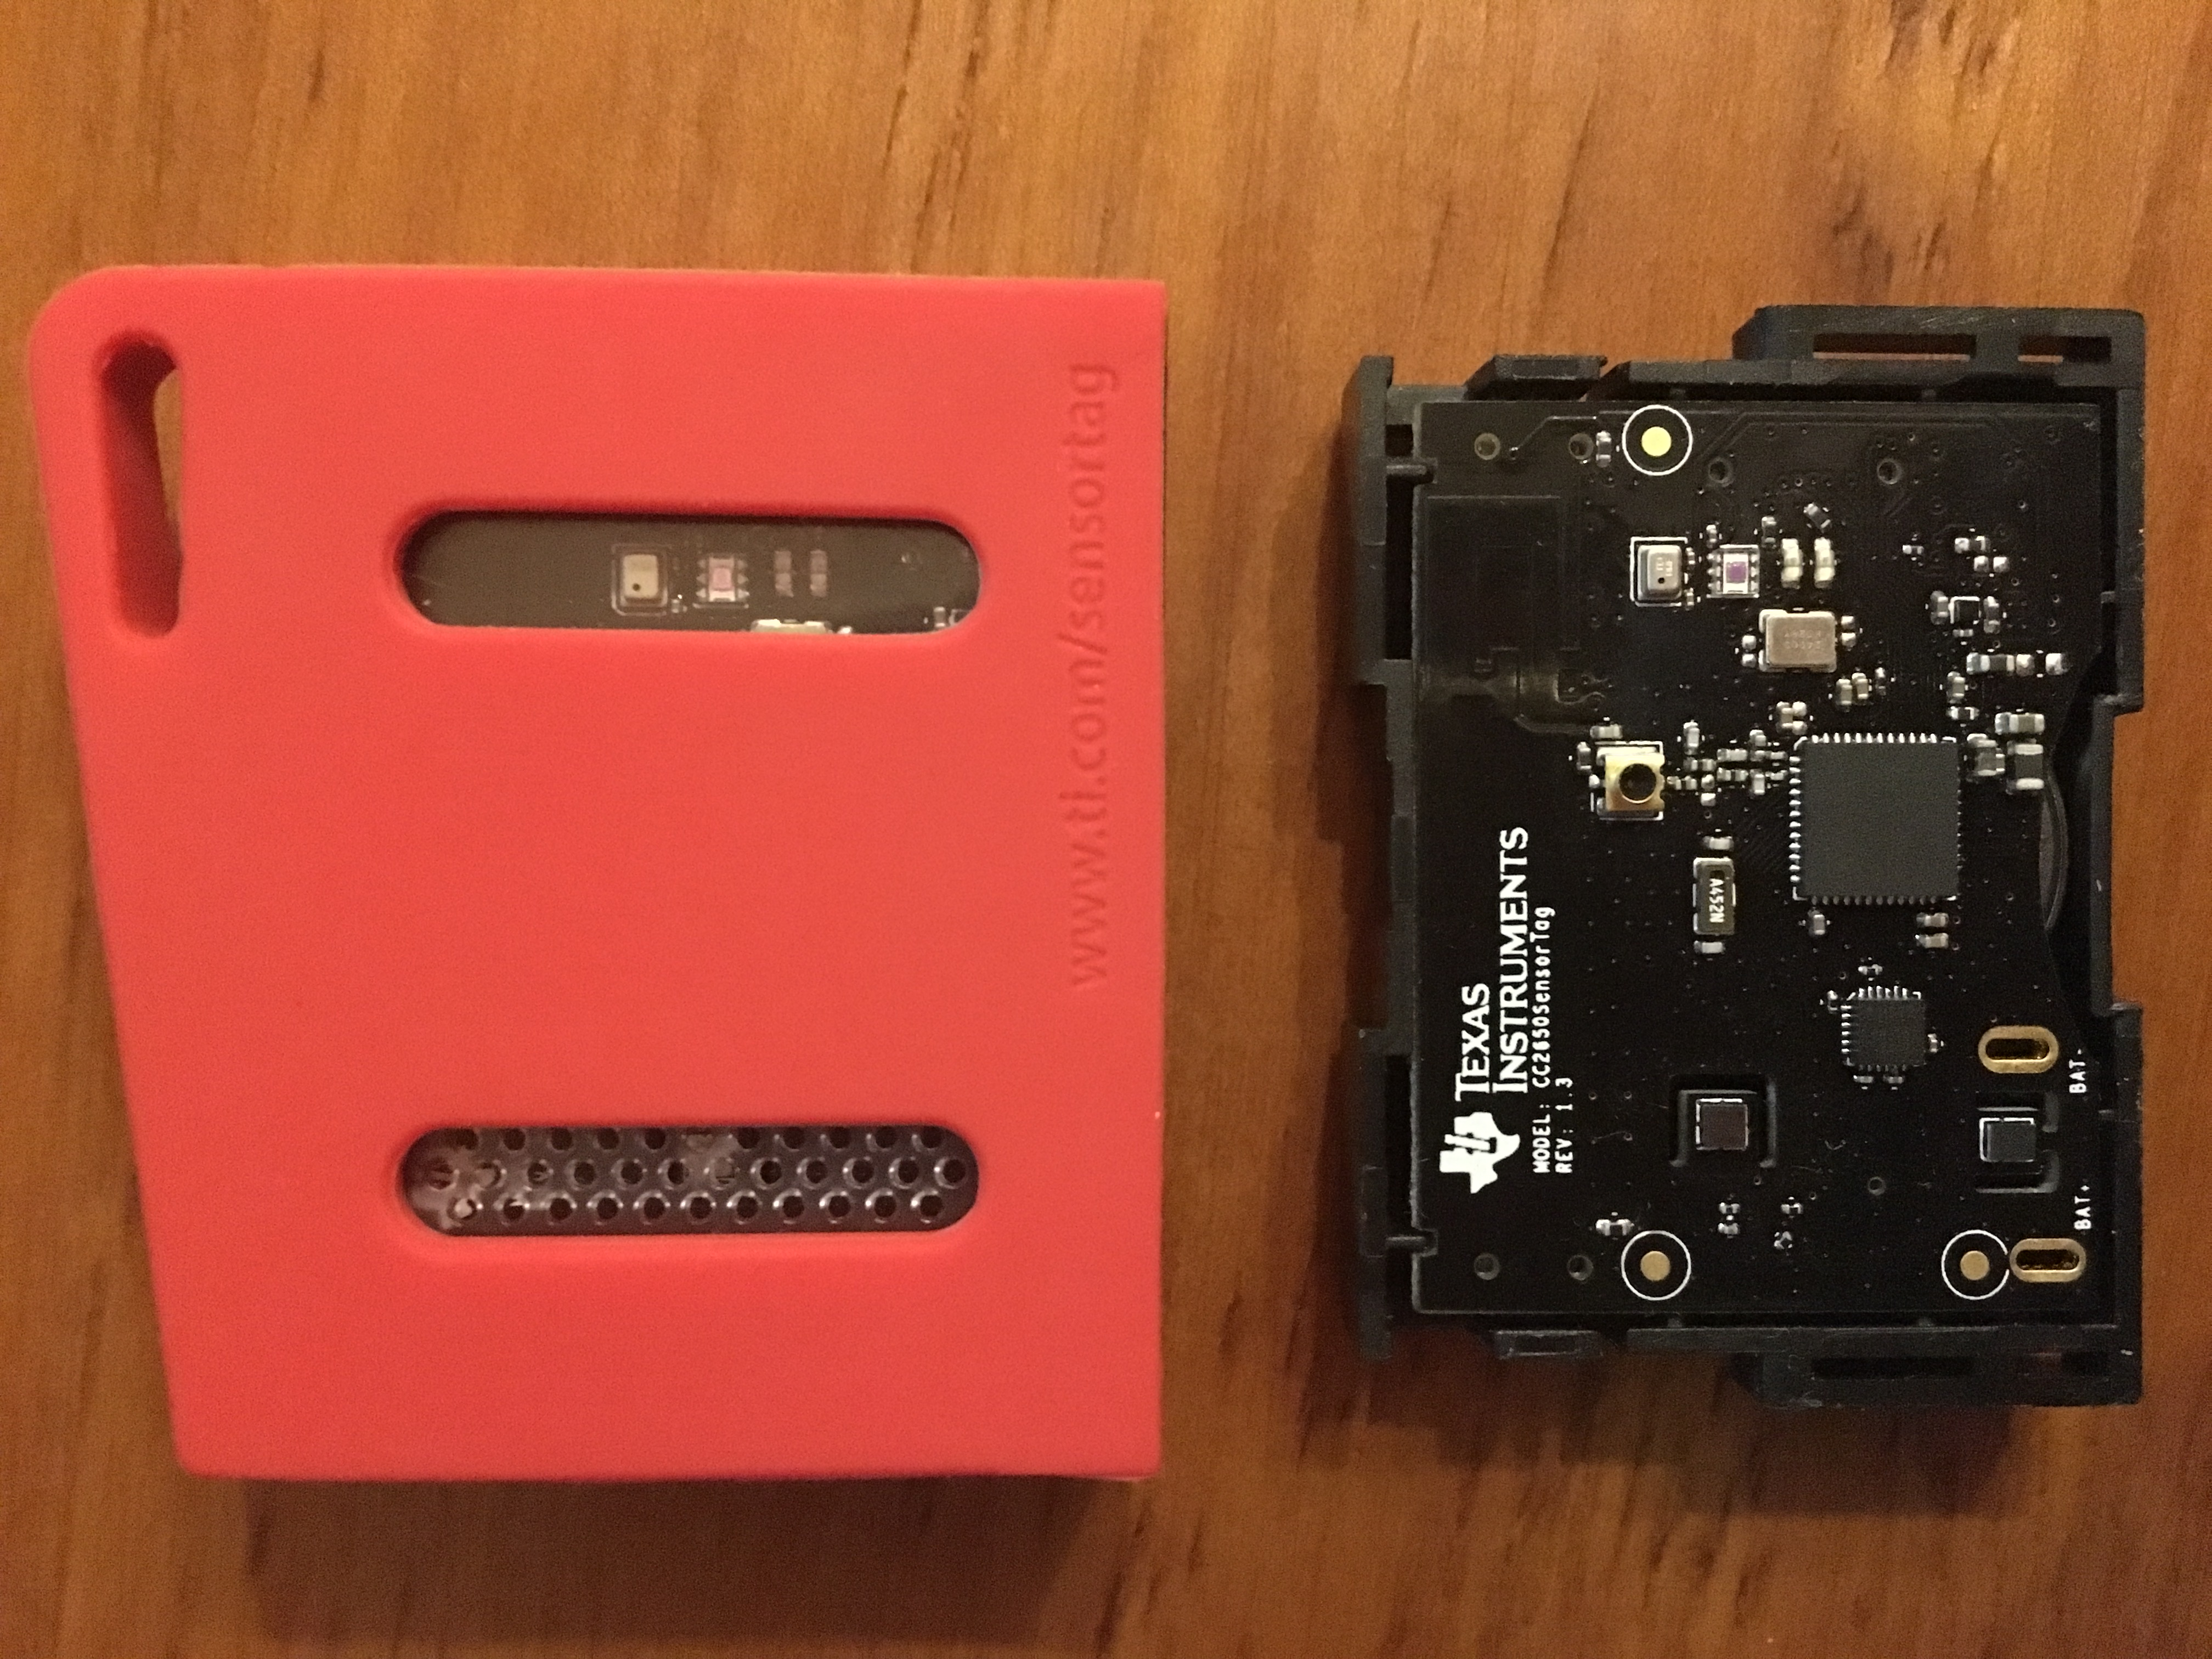
\includegraphics[width=0.5\linewidth]{4.Chapter/beacon.jpg}
	\caption[TI cc2650stk sensortag]{TI cc2650stk sensortag}
	\label{fig:beacon}
\end{figure}

\section{Server}
\label{sec:server}

The webserver was implement in Python 3 programming language. The program implements a simple tcp server capable of receiving multiple request at the same time. Each request starts with information sent from an application which include a pair of MAC address and associated RSSI value for each ble device that the same application found. Afterwards the list of pairs is filtered in order to remove any existant devices that are not present in the server's database of devices.

Each server has a database that includes only ble devices. An entry (description of a device) in this database is composed by the device's mac address, its longitude and latitude and its building, floor and room name. In addition to the database, a server when initiated can store additional location info such as the server's street, number, zipcode, city and country, allowing this information to be transmited to the client in order to offer an additional level of location description to the user. The whole location specific information can be visualised in figure ~\ref{fig:AppMenu}.

Upon having filtered the initial list of pairs, the Cell of Origin (CoO) technique is applied by verifying which of the devices produced a stronger signal on the receptor. Upon obtaining the closest device an answer is sent to the application containing all of the information associated to the server and the selected device.


- Describe the Database ( insert image example of database with a few entries?? )

- Mention capability to Insert aditional info, at the moment it displays geocoding on pop up menu in figure ~\ref{fig:AppMenu}.


\section{Application}
\label{sec:app}


The Smartphone application was developed for Android using the Android Studio IDE. The Application is divided in two primary functional blocks, the Mock location Provider and the Google Maps Integrated Display, as can be visualised in figure \ref{fig:implementation}.

The Mock Location Provider is implemented as if it was a Location provider, such as GPS. The application functions works as a listener to a Location provider, in this case it listens to the Mock Provider that was implemented. By implementing the whole process of obtaining a location inside a service (the mock provider) , a new level of abstraction is added to the application. As such, whenever the application is signalled to obtain the user's current location, a request is made to the associated location provider and the application only need to listen for the answer that eventually arrives.

\begin{figure}
	\centering
		\includegraphics[width=0.5\linewidth]{4.Chapter/RequestLocation.png}
	\caption[Mock Location Provider Workflow]{Mock Location Provider Workflow}
	\label{fig:MockProvider}
\end{figure}

The Mock Location Provider incorporates the first three steps present in figure ~\ref{fig:MockProvider}, which will now be explored individually. The first step indicates the gathering of information of the surroundings of the user's device. When a request is made to the provider, a scan for nearby bluetooth low energy devices is made which will put the smartphone in a state of listening for incoming \ac{BLE} advertisement packets for half a second ( NEED TO VERIFY VALUE AND JUSTIFY, THERE WAS A PAPER ON THIS TODO). During this scanning period, each time a device is found, the advertisement is registered in a list, which have a duplication prevention mechanism implemented. Once the period is over, the provider has available a list of all the \ac{BLE} devices within range.   

The second step involves taking the created list of devices, obtain a server address and forward the same list to it. Once the first step is completed, the provider will analyse each entry at a time. For each device the provider will attempt to respond to the caught advertisement packet, resulting in a created connection.  Once the connection is created the provider asks for the available services of the paired device. Upon receiving an answer, the list of services is swoop while looking for the service with the wanted UUID. If the device doesn't have the UUID that the provider is looking for, it can assume that the paired \ac{BLE} is not a beacon of our system, as such the connection is terminated. When the provider identifies that the device has the system's UUID, it requests the device to provide the service's existent characteristics. The provider will receive a list composed of the service's characteristics and it will search in it for the system's characteristics UUID, the one which contains the device's server's address. This search has the objective of confirming that the service existent in this device is indeed the one that was implemented for the system and not a device with another service that happened to have the same UUID. For any service outside those that are documented in the Bluetooth Special Interest Group (SIG), who have a specific UUID attached to them, the UUID is generated randomly and as such there is a small chance of collision. Once the wanted characteristic is found, the provider requests the device to read its value and stores the received value in a list. This list will contain the servers of the devices that were found, and for each address there will be a list corresponding to each device , and their corresponding rssi values, from the same owner. In order to quicken the previously described process, the provider keeps in cache the most recent contacted devices. Before attempting a connection, the provider confirms that the device isn't found in cache and when finishing a process, the associated device is inserted into the cache.

When every device has been contacted, a voting system is actioned which will decide from the list of servers which one it will send the collected information to. The voting system uses an exponential function in order to attribute a weight to each server. %INSERT FUNCTION AND EXPLAINATION.

The voting system was implemented with the objective providing a thin security layer by allowing multiple devices of the same server to overcome a single attacker's device which happened to be close to the user. After obtaining each server's values, the one with the highest value is chosen and sent the list with all the devices. 

The Third step involves a simple client/server tcp interaction. The application starts off by formulating the message that it will later on send to the server, this message includes all pairs of device mac address and its associated rssi value captured by the application on the first step. Once the message is computed, the application attempts to create a connection with the server at the chosen address at the end of step two. With the connection established, the message is forwarded to the server and the application is put onto blocked state where it awaits for an answer. Upon arrival, the answer received is checked for valid location, its information is process and the connection is terminated. The information contained inside the received message, which was described in section ~\ref{sec:server}, is then processed into the adequate class capable of storing a geographic location and the same is broadcasted from the mock location provider to its listener. 



One of the current limitations of the android API that deals with \ac{BLE} is that the interface on the smartphone that is used to connect with a device has a fixed timeout time.  %MIGHT JUST NEED TO BE IMPROVED TODO


The Google Maps Integrated display is implemented using the Google Maps Android API. By using Google Maps it was possible to alleviate the weight on application since there wasn't need implement file transfer of indoor building's maps from each dedicated server to each request, which alleviated the servers as well since there was no need to store its associated building's maps on it. Managing the maps was something that was as well fortunately unnecessary and as such all these features were provided by google maps service. By making this development choice, the system as whole became closer to the desired generic approach while making possible for seamless transition between indoor/outdoor maps. The only imposed restriction is related to the addiction of new indoor maps onto the google maps, which is possible and well documented but dependent on a third party.

The Fourth step is called when the application receives a proper location from the request made onto the location provider. With the device's location known, a marker is placed on the map with the obtain coordinates (longitude, latitude), the camera is moved in order to be centralised on the position and fully displaying the indoor level map, and the menu visible on figure ~\ref{fig:AppMenu} is updated with the information that is bundled with the received location. In order to show the correct level on a multi level building, the "floor" information present in the menu is utilised. The API allows for obtaining a list of existent levels on which the maps' camera is focused and as such it's possible to find out to which level the provided location belongs and make so that the application shows it.

The pop-up menu was implemented to demonstrate the capacity of providing additional information associated with each location, be it geo-location taxonomy as it is currently implemented or possibly a description of the located room, an hyperlink of some sort or any other type of data that someone implemented this system would like to provide to its users.  

The final state of the implemented system can be visualised in figure ~\ref{fig:AppFocus} and figure ~\ref{fig:AppMenu}. The first displays the case of obtaining a location, where the marker has been placed and the camera zoomed

\begin{figure}
	\centering
		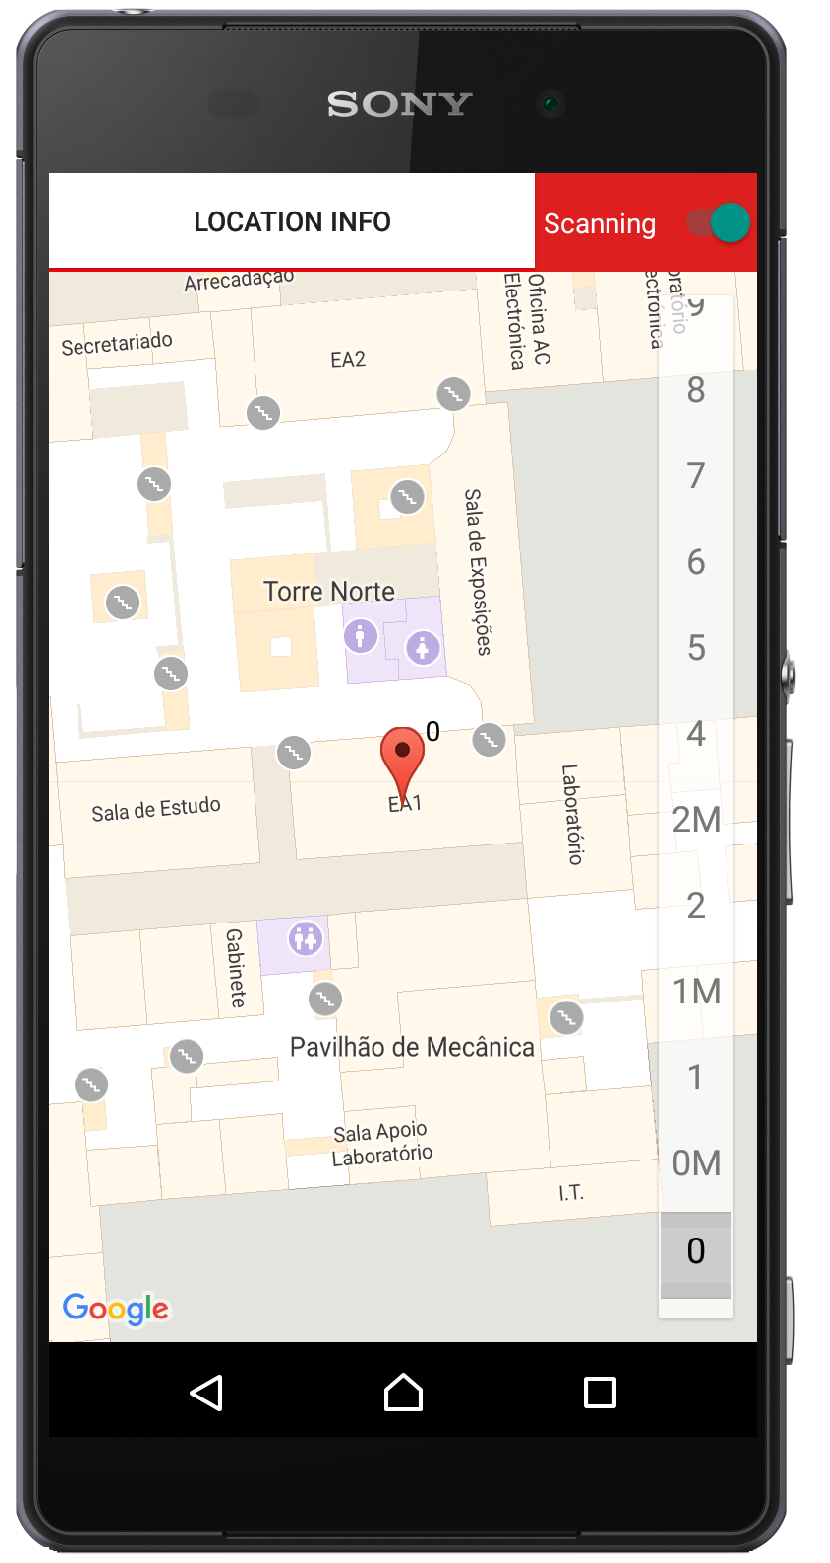
\includegraphics[width=0.5\linewidth]{4.Chapter/app_focused.png}
	\caption[Application screen showing a focused location on a room]{Application screen showing a focused location on a room}
	\label{fig:AppFocus}
\end{figure}

\begin{figure}
	\centering
		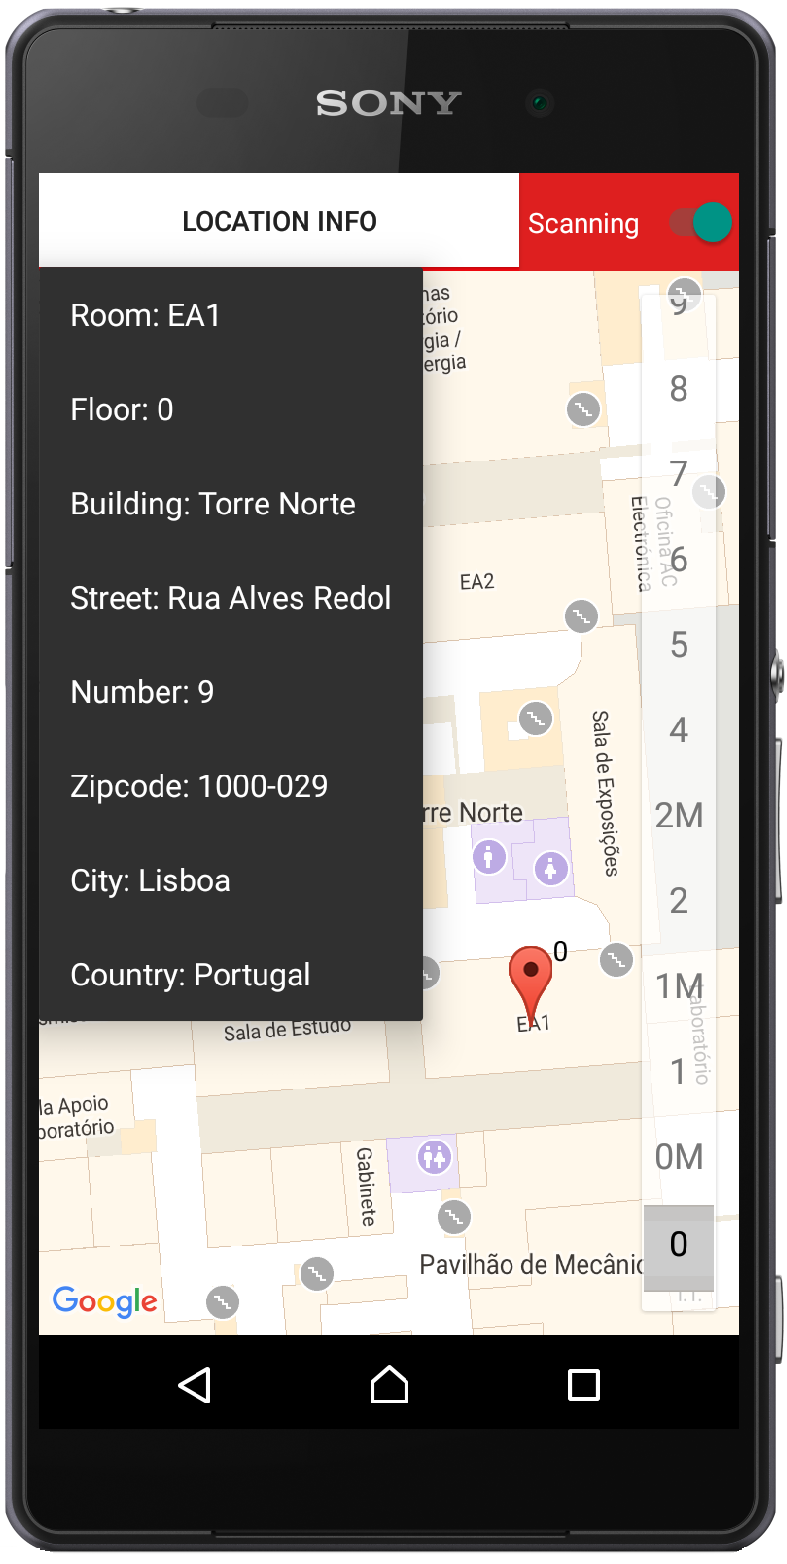
\includegraphics[width=0.5\linewidth]{4.Chapter/app_focused_menu.png}
	\caption[Application screen showing additional information of location]{Application screen showing additional information of location}
	\label{fig:AppMenu}
\end{figure}



\cleardoublepage
